\documentclass{article}

\usepackage{amsmath,amssymb}
\usepackage{fullpage}
\usepackage{enumerate}
\usepackage{hyperref}
\usepackage{graphicx}
\graphicspath{{../logos/}}


\begin{document}

\setlength{\tabcolsep}{6pt}
\begin{center} \begin{tabular}{cccc}
	
\includegraphics[height=56pt]{SAMF_logo.jpg} &
	
\includegraphics[height=56pt]{SAICA_logo.jpg} &
	
\includegraphics[height=56pt]{OM_Logo_Stacked_Vignette_on_White_RGB.jpg} &
	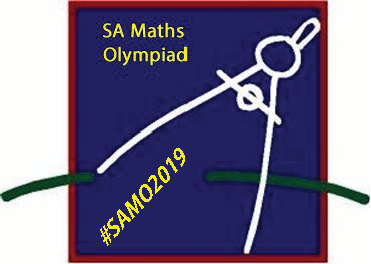
\includegraphics[height=56pt]{SAMO2019.png}
\end{tabular} \end{center}


\bigskip


\begin{center}
	\textbf{\Large Senior January Monthly Problem Set Solutions}
\end{center}

\begin{enumerate}

\medskip
\item % PAMO Shortlist 2019
{\itshape On the board, we write the integers $1, 2, 3, \dots, 2019$.
At each minute, we pick two numbers on the board $a$ and $b$, erase them, and write down the number $s(a + b)$ instead where $s(n)$ denotes the sum of the digits of the integer $n$.
Let $N$ be the last number remaining on the board.
\begin{enumerate}
	\item Is it possible that $N = 19$?
	\item Is it possible that $N = 15$?
\end{enumerate}}
Solution.
\\ {Since $10^{n} \equiv 1 \pmod 3$ for all non-negative integers $n$, we have that $s(n) \equiv n \pmod 3$ and so replacing $a$ and $b$ with $s(a+b)$ does not change the sum of the numbers on the board in mod 3. 
\\ Now $1 + 2 +... + 2019 = \frac{(2019)(2020)}{2} \equiv 0 \pmod 3$ but $19 \not\equiv 0 \pmod 3$ so we cannot have $N=19$ as the last number on the board. 
\\
\\ We now show that we can in fact get to $15$. 
\\ For each $k \neq \{1010, 906\}$, replace the numbers $k$ and $2020-k$ with $s(k + 2020-k) = s(2020)$ = $4$. So remaining on the board now is $906, 1114, 1010$ and $1008$ $4$s. Now taking the $4$s in pairs and applying the procedure gives $504$ $8$s, taking these in pairs gives $252$ $7$s, and taking these $7$s in pairs gives $126$ $5$s and again taking these $5$s as pairs gives $63$ $1$s. So we have left $906, 1114, 1010$ and $63$ $1$s. Now apply the procedure in $1114$ and $1010$ to get $s(2125)=9$ and remain with $9, 906$ and $63$ $1$s. Now from the $63$ $1$s, we can make $7$ $9$s by taking $1$s and applying the procedure until we get to a $7$ then we stop and take a $1$ that has not been used. We then have $8$ $9$s and $906$ left on the board. Since $s(9 + 9) = s(18) = 9$, we can apply this procedure to the $9$s until just one $9$ remains. Finally, we combine this $9$ with the $906$ to get $s(906 + 9) = s(915) = 15$.} 
\\ \\Remark. {\itshape The steps used to get to 15 are not unique.} 


\medskip
\item % Baltic Way 2009 Problem 8
{\itshape For which positive integers $n$ is it possible to divide the set of numbers $\{n, n+1, n+2, \dotsc, n+8\}$ into two disjoint sets $A$ and $B$ such that the product of the numbers in $A$ is equal to the product of the numbers in $B$?}



\medskip
\item % Liam
{\itshape Let $M$ be a positive integer, and let $S$ denote the set of finite sequences of positive integers less than or equal to $M$, including the empty sequence of length zero, which we denote as $\mathbf{0}$.
Also, for a sequence $\mathbf{x} = (x_1, x_2, \dotsc, x_n)$ let $\overline{\mathbf{x}}$ denote the reverse sequence $\overline{\mathbf{x}} = (x_n, x_{n-1}, \dotsc, x_1)$.

Define a function $d$ from $S$ to the integers as follows:
\begin{itemize}
\item $d(\mathbf{0}) = 0$.
\item If $\mathbf{x} = (x_1, x_2, \dotsc, x_n)$ is a sequence of positive length, let $m$ be the largest integer such that $x_1 +x_2 +\dotsb +x_m \leq M$, and let $\mathbf{x}'$ denote the rest of the sequence: $\mathbf{x}' = (x_{m+1}, \dotsc, x_n)$.
Then $d(\mathbf{x}) = 1 +d(\mathbf{x}')$.
\end{itemize}
Show that $d(\mathbf{x}) = d(\overline{\mathbf{x}})$.}



\medskip
\item
{\itshape Let $ABCD$ be a cyclic quadrilateral with its diagonals intersecting at $E$.
Let $M$ be the midpoint of $AB$.
Suppose that $ME$ is perpendicular to $CD$.
Show that either $AC$ is perpendicular to $BD$ or $AB$ is parallel to $CD$.}



\medskip
\item % IMO 2008 Shortlist C3
{\itshape We have done it! We have planted an infinite number of trees on the vertices of an infinite regular grid, one for each vertex. Let $T$ be a positive integer. 
We define a {\itshape T-forest} as a set of trees such that for any two trees in the $T$-forest, there exists another tree planted in the grid such that the area of the triangle with these three trees as vertices is $T$.

What is the smallest $T$ such that our $T$-forest has more than $200$ trees?}



\medskip
\item % IMO 2009 Shortlist N4
{\itshape Given a series $t_1, t_2, \dotsc, t_n$ such that 
\[ t_{k + 1} = \frac{t_k^2 + 1}{t_{k-1} + 1} - 1 \quad \forall \ k \in \{2, 3, \dots, n-1\}. \]
For which $n \in \mathbb{N}$ does there exist a $t_1$ and $t_2$ such that $t_i \in \mathbb{N}$ for all $i \in \{1, 2, 3, \dotsc, n\}$?}



\medskip
\item % Modified Iran TST 2018 Q6
{\itshape Let $AC$ and $BD$ be two chords of a circle $\Gamma$ that intersect at $X$ in the interior of $\Gamma$.
Let $\Gamma_1$ and $\Gamma_2$ be circles that are mutually tangent at $X$ and are tangent to $\Gamma$ at $P$ and $Q$.
Let $\omega$ be a circle tangent to $\Gamma_1$ and $\Gamma_2$ at $X$ that intersects the chords $AB$ and $CD$ at $M$ and $N$ respectively.
Prove that
\[
	\frac{MP}{MQ} = \frac{NP}{NQ} \implies \angle AXM = \angle DXN.
\]}



\medskip
\item % The Andrew and The Dylan
{\itshape Let $n$ be a positive integer greater than $1$, and consider a circle of radius $1$ in which is inscribed a regular $n$-gon $P$ with vertices labelled from $1$ to $n$ in that order.
Consider the set $S$ of positive divisors of $n$, and the convex polygon $G$ formed by the points of $P$ with labels in $S$.
If the area of $G$ is denoted by $|G|$, show that
\[ 
	|G| < \frac{3}{2}.
\]}


\end{enumerate}

\end{document}